\documentclass[10pt]{article}
\usepackage{preamble}

\def\FS{Formelsammlung}
\def\Fach{Felder, Wellen und Leitungen}
\title{\FS \\ \Fach}
\date{\today}
\def\Semester{Wintersemester 23/24}
\IfFileExists{info.tex}
{
   \input{info.tex}
}
{
   \author{\href{https://www.youtube.com/watch?v=yMR45cZbvDw}{Die Prinzen - Alles nur geklaut}}
   \def\MatNr{MATNR}
}

\begin{document}

\pagenumbering{gobble}
\begin{titlepage}
	\thispagestyle{empty}

	\begin{center}
		\includegraphics[width=0.7\textwidth]{OTHR_OTHR_Logo}\\
		\vspace*{\stretch{1}}
		\Huge
		\textsc{\MyTitle}\\
		\vspace*{\stretch{0.25}}
		\large
		\textbf{\Semester}\\
		{\small
		nach Vorlesung von Prof. Stücke und Prof. Sattler}

		\vspace*{\stretch{0.5}}
    Erstellt von\\ Max Forstner, \href{https://ayhamcloud.de/}{Ayham
    Alhulaibi}, \href{https://github.com/Vibeskanzler}{Tony Pham}  und Johannes
    Rothe\\


		\vspace*{\stretch{2}}
		{\renewcommand{\arraystretch}{1.5}
			\begin{tabular}{l l}
				Name:            & \hspace{4cm}\MyAuthor \\
				Matrikelnummer:  & \hspace{4cm}\MatNr    \\
				Letzte Änderung: & \hspace{4cm}\MyDate   \\
				Lizenz:          & \hspace{4cm}GPLv3
			\end{tabular}
		}
		\vspace*{\stretch{1}}
		\vspace*{\stretch{2}}


	\end{center}
\end{titlepage}

\newpage
\tableofcontents
\clearpage

\pagestyle{fancy}
\lhead{\MyAuthor}
\rhead{\Semester}
\cfoot{\vspace{-20pt}\thepage}
\pagenumbering{arabic}
% \setlength{\columnsep}{1pt}
\raggedcolumns

\begin{multicols*}{2}
	\section{Grundlagen}
\subsection{mathematische}
\subsubsection*{Divergenz/Rotation/Gradient}

$\opdiv$: macht aus einem Vektor ein Skalar.\\
$\operatorname{rot}$: bildet ein Vektor auf Vektorfeld ab.\\
$\opgrad$: bildet ein Skalar-/Gradientenfeld in ein Vektorfeld ab.
Zeigt Richtung stärkster Zunahme des Feldes.
\begin{align*}
    \opdiv \vec{G}  &= \nabla \cdot \vec{G} = \dfrac{\partial G_x}{\partial x} + \dfrac{\partial G_y}{\partial y} + \dfrac{\partial G_z}{\partial z}\\
                                &= 0 \quad\Rightarrow \textnormal{Volumen}\\
                                &> 0 \quad\Rightarrow \textnormal{Quelle}\\
                                &< 0 \quad\Rightarrow \textnormal{Senke}\\
    \arraycolsep=1.0pt\def\arraystretch{2.0}
    \operatorname{rot} \vec{G}  &= \nabla \times \vec{G} =
        \begin{pmatrix}
            \dfrac{\partial G_z}{\partial y} - \dfrac{\partial G_y}{\partial z} \\
            \dfrac{\partial G_x}{\partial z} - \dfrac{\partial G_z}{\partial x} \\
            \dfrac{\partial G_y}{\partial x} - \dfrac{\partial G_x}{\partial y} \\
        \end{pmatrix}\\                       
    \arraycolsep=1.0pt\def\arraystretch{2.0}
    \opgrad G       &= \nabla \cdot G =
        \begin{pmatrix}
            \dfrac{\partial G}{\partial x} \\
            \dfrac{\partial G}{\partial y} \\
            \dfrac{\partial G}{\partial z} \\
        \end{pmatrix}                                      
\end{align*}

\subsubsection*{Nabla Operator}

\[
    \nabla = \vec{\nabla} = \left( \dfrac{\partial G}{\partial x},
    \dfrac{\partial G}{\partial y}, \dfrac{\partial G}{\partial z} \right)
\]

Feldänderung bei Bewegung
\begin{align*}
    \Delta G & = \dfrac{\partial G}{\partial x} \Delta x + \dfrac{\partial G}{\partial y} \Delta y + \dfrac{\partial G}{\partial z} \Delta z \\
             & = dG = \opgrad G \cdot d \vec{s}
\end{align*}



\subsection{Randbedingung}
\begin{tabularx}{0.45\textwidth}{>{\hsize=.3\hsize}X|>{\hsize=.7\hsize}X}
    Dirichlet-RB & Funktion nimmt an den Rändern einen bestimmten Wert an (Bsp.: $\rho_r = 5V$)\\
    \hline
    Neumann-RB &  Die Normalableitung der Fkt. nimmt an den Rändern einen bestimmten Wert an\\
\end{tabularx}

\subsection{Begriffe}
\begin{tabularx}{0.45\textwidth}{>{\hsize=.2\hsize}X|>{\hsize=.4\hsize}X|>{\hsize=.4\hsize}X}
        & Begriff & Beschreibung \\
    \hline
    $\rho$ & Raumladungsdichte &  \\
\end{tabularx}


\subsection{Kartesische Koordinaten}
Einheitsvektoren:   $\quad \vec{e_{x}}, \vec{e_{y}}, \vec{e_{z}}$\\ 
Rechtssystem:       $\quad \vec{e_{x}} \times \vec{e_{y}}=\vec{e_{z}}$\\
Linienelemente:     $\quad d s=\sqrt{d x^{2}+d y^{2}+d z^{2}}$\\
Nabla Operator:     $\quad \nabla=\frac{\partial}{\partial x} \vec{e_{x}}+\frac{\partial}{\partial y} \vec{e_{y}}+\frac{\partial}{\partial z} \vec{e_{z}}$\\
Gradient:           $\quad \opgrad \varphi \equiv \nabla \varphi=\frac{\partial \varphi}{\partial x} \vec{e_{x}}+\frac{\partial \varphi}{\partial y} \vec{e_{y}}+\frac{\partial \varphi}{\partial z} \vec{e_{z}}$\\
Divergenz:          $\quad \opdiv \vec{D} \equiv \nabla \vec{D}=\frac{\partial D_{x}}{\partial x}+\frac{\partial D_{y}}{\partial y}+\frac{\partial D_{z}}{\partial z}$\\
Rotation:           $\quad \operatorname{rot} \vec{E} \equiv \nabla \times \vec{E} =$\\
                        $\left[\frac{\partial E_{z}}{\partial y}-\frac{\partial E_{y}}{\partial z}\right] \vec{e_{x}}+\left[\frac{\partial E_{x}}{\partial z}-\frac{\partial E_{z}}{\partial x}\right] \vec{e_{y}}+\left[\frac{\partial E_{y}}{\partial x}-\frac{\partial E_{x}}{\partial y}\right] \vec{e_{z}}$\\
Laplace Operator:   $\quad \Delta=\frac{\partial^{2} \ldots}{\partial x^{2}}+\frac{\partial^{2} \ldots}{\partial y^{2}}+\frac{\partial^{2} \ldots}{\partial z^{2}}$\\
\begin{align*}
    &\Delta \vec{E} = \opgrad \opdiv \vec{E}-\operatorname{rot} \operatorname{rot} \vec{E} =\Delta E_{x} \vec{e_{x}}+\Delta E_{y} \vec{e_{y}}+\Delta E_{z} \vec{e_{z}}=\\
                   &= \left[\frac{\partial^{2} E_{x}}{\partial x^{2}}+\frac{\partial^{2} E_{x}}{\partial y^{2}}+\frac{\partial^{2} E_{x}}{\partial z^{2}}\right] \vec{e_{x}}+\left[\frac{\partial^{2} E_{y}}{\partial x^{2}}+\frac{\partial^{2} E_{y}}{\partial y^{2}}+\frac{\partial^{2} E_{y}}{\partial z^{2}}\right] \vec{e_{y}}\\
                   &+ \left[\frac{\partial^{2} E_{z}}{\partial x^{2}}+\frac{\partial^{2} E_{z}}{\partial y^{2}}+\frac{\partial^{2} E_{z}}{\partial z^{2}}\right] \vec{e_{z}}
\end{align*}


\subsection{Zylinderkoordinaten}
Variablen:          $\quad r, \alpha, z$\\
Einheitsvektoren:   $\quad \vec{e_{r}}, \vec{e_{\alpha}}, \vec{e_{z}} \quad$\\
Rechtssystem: $\vec{e_{r}} \times \vec{e_{\alpha}}=\vec{e_{z}}$\\
% Zusammenhang mit rechtwinkligen Koordinaten:
% \begin{align*}
%     x&=r \cos \alpha \quad r=\sqrt{x^{2}+y^{2}} \quad d r=d x \cos \alpha+d y \sin \alpha\\
%     y&=r \sin \alpha \quad \alpha=\arctan \frac{y}{x} \quad r d \alpha=d y \cos \alpha-d x \sin \alpha\\
%     z&=z \quad z=z \quad d z=d z
% \end{align*}
Linienelemente:     $\quad d s=\sqrt{d r^{2}+r^{2} d \alpha^{2}+d z^{2}}$\\
Volumenelemente:    $\quad d v=r d r d \alpha d z$\\
Nabla Operator:     $\quad \nabla=\frac{\partial}{\partial r} \vec{e_{r}}+\frac{1}{r} \frac{\partial}{\partial \alpha} \vec{e_{\alpha}}+\frac{\partial}{\partial z} \vec{e_{z}}$\\
Gradient:           $\quad \opgrad \varphi \equiv \nabla \varphi=\frac{\partial \varphi}{\partial r} \vec{e_{r}}+\frac{1}{r} \frac{\partial \varphi}{\partial \alpha} \vec{e_{\alpha}}+\frac{\partial \varphi}{\partial z} \vec{e_{z}}$\\
Divergenz:          $\quad \opdiv \vec{D} \equiv \nabla \vec{D}=\frac{1}{r} \frac{\partial\left(r \vec{D}_{r}\right)}{\partial r}+\frac{1}{r} \frac{\partial \vec{D}_{\alpha}}{\partial \alpha}+\frac{\partial \vec{D}_{z}}{\partial z}$\\
Rotation:           $\quad \operatorname{rot} \vec{E} \equiv \nabla \times \vec{E}=\left[\frac{1}{r} \frac{\partial E_{z}}{\partial \alpha}-\frac{\partial E_{\alpha}}{\partial z}\right] \vec{e_{r}}+\left[\frac{\partial E_{r}}{\partial z}-\frac{\partial E_{z}}{\partial r}\right] \vec{e_{\alpha}}+\left[\frac{1}{r} \frac{\partial\left(r E_{\alpha}\right)}{\partial r}-\frac{1}{r} \frac{\partial E_{r}}{\partial \alpha}\right] \vec{e_{z}}$\\
Laplace Operator:   $\quad \Delta = \frac{1}{r}\frac{\partial \left(r \frac{\partial \ldots}{\partial r}\right)}{\partial r} + \frac{1}{r^2}\frac{\partial^2 \ldots}{\partial \alpha^2} + \frac{\partial^2 \ldots}{\partial z^2}$\\
\begin{align*}
    \vec{E} =& \left[\Delta E_{r}-\frac{2}{r^{2}} \frac{\partial E_{\alpha}}{\partial \alpha}-\frac{E_{r}}{r^{2}}\right] \vec{e_{r}}\\
             &+\left[\Delta E_{\alpha}+\frac{2}{r^{2}} \frac{\partial E_{r}}{\partial \alpha}-\frac{E_{\alpha}}{r^{2}}\right] \vec{e_{\alpha}}+\left[\Delta E_{z}\right] \vec{e_{z}}
\end{align*}


\subsection{Kugelkoordinaten}
Variablen:          $\quad r, \vartheta, \alpha$\\
Einheitsvektoren:   $\quad \vec{e_{r}}, \vec{e_{\vartheta}}, \vec{e_{\alpha}}$\\
Rechtssystem:       $\quad \vec{e_{r}} \times \vec{e_{\vartheta}}=\vec{e_{\alpha}}$\\
% Zusammenhang mit rechtwinkligen Koordinaten:
% \begin{align*}
%     x&=r \sin \vartheta \cos \alpha \quad r=\sqrt{x^{2}+y^{2}+z^{2}} \quad d r=d x \sin \vartheta \cos \alpha+d y \sin \vartheta \sin \alpha+d z \cos \vartheta\\
%     y&=r \sin \vartheta \sin \alpha \quad \alpha=\arctan \frac{y}{x} \quad r \sin \vartheta d \alpha=d y \cos \alpha-d x \sin \alpha\\
%     z&=r \cos \vartheta \quad \vartheta=\arctan \frac{\sqrt{x^{2}+y^{2}}}{z} \quad r d \vartheta=d x \cos \vartheta \cos \alpha+d y \cos \vartheta \sin \alpha-d z \sin \vartheta
% \end{align*}
Linienelement:      $\quad d s=\sqrt{d r^{2}+r^{2} \sin ^{2} \vartheta d \alpha^{2}+r^{2} d \vartheta^{2}}$\\
Volumenelement:     $\quad d v=r^{2} \sin \vartheta d r d \vartheta d \alpha$\\
Nabla Operator:     $\quad \nabla=\frac{\partial}{\partial r} \vec{e_{r}}+\frac{1}{r} \frac{\partial}{\partial \vartheta} \vec{e_{\vartheta}}+\frac{1}{r \sin \vartheta} \frac{\partial}{\partial \alpha} \vec{e_{\alpha}}$\\
Gradient:           $\quad \opgrad \varphi \equiv \nabla \varphi=\frac{\partial \varphi}{\partial r} \vec{e_{r}}+\frac{1}{r} \frac{\partial \varphi}{\partial \vartheta} \vec{e_{\vartheta}}+\frac{1}{r \sin \vartheta} \frac{\partial \varphi}{\partial \alpha} \vec{e_{\alpha}}$\\
Divergenz:          $\quad \opdiv \vec{D} \equiv \nabla \vec{D}=\frac{1}{r^{2}} \frac{\partial\left(r^{2} D_{r}\right)}{\partial r}+\frac{1}{r \sin \vartheta} \frac{\partial\left(\sin \vartheta \cdot D_{\vartheta}\right)}{\partial \vartheta}+\frac{1}{r \sin \vartheta} \frac{\partial D_{\alpha}}{\partial \alpha}$\\
Rotation:           
\begin{align*}
    \operatorname{rot} \vec{E} &\equiv \nabla \times \vec{E}= \frac{1}{r \sin \vartheta}\left[\frac{\partial\left(\sin \vartheta \cdot E_{\alpha}\right)}{\partial \vartheta}-\frac{\partial E_{\vartheta}}{\partial \alpha}\right] \vec{e_{r}}\\
        +&\frac{1}{r}\left[\frac{1}{\sin \vartheta} \frac{\partial E_{r}}{\partial \alpha}-\frac{\partial r E_{\alpha}}{\partial r}\right] \vec{e_{\vartheta}}+\frac{1}{r}\left[\frac{\partial\left(r E_{\vartheta}\right)}{\partial r}-\frac{\partial E_{r}}{\partial \vartheta}\right] \vec{e_{\alpha}}
\end{align*}
Laplace Operator:   $\quad \Delta=\frac{1}{r^{2}} \frac{\partial\left(r^{2} \frac{\partial . .}{\partial r}\right)}{\partial r}+\frac{1}{r^{2} \sin \vartheta} \frac{\partial\left(\sin \vartheta \frac{\partial . \ddot{ }}{\partial \vartheta}\right)}{\partial \vartheta}+\frac{1}{r^{2} \sin ^{2} \vartheta} \frac{\partial^{2} . .}{\partial \alpha^{2}}$
Laplace Operator in Kugelkoordinaten, angewandt auf einen Vektor:
\begin{align*}
    \Delta \vec{E} &=\left[\Delta E_{r}-\frac{2}{r^{2}} E_{r}-\frac{2}{r^{2} \sin \vartheta} \frac{\partial\left(\sin \vartheta \cdot E_{\vartheta}\right)}{\partial \vartheta}-\frac{2}{r^{2} \sin \vartheta} \frac{\partial E_{\alpha}}{\partial \alpha}\right] \vec{e_{r}} \\
    &+\left[\Delta E_{\vartheta}-\frac{E_{\vartheta}}{r^{2} \sin ^{2} \vartheta}+\frac{2}{r^{2}} \frac{\partial E_{r}}{\partial \vartheta}-\frac{2 \cot \vartheta}{r^{2} \sin \vartheta} \frac{\partial E_{\alpha}}{\partial \alpha}\right] \vec{e_{\vartheta}} \\
    &+\left[\Delta E_{\alpha}-\frac{E_{\alpha}}{r^{2} \sin ^{2} \vartheta}+\frac{2}{r^{2} \sin \vartheta} \frac{\partial E_{r}}{\partial \alpha}+\frac{2 \cot \vartheta}{r^{2} \sin \vartheta} \frac{\partial E_{\vartheta}}{\partial \alpha}\right] \vec{e_{\alpha}}
\end{align*}

 

\subsection{Vergleich/Umrechnung}
\begin{tabularx}{0.45\textwidth}{>{\hsize=.46\hsize}X|>{\hsize=.27\hsize}X|>{\hsize=.27\hsize}X}
    Kart. & Zyl. & Kug.\\
    \specialrule{1.5pt}{0pt}{0pt}
    $x$                                 & $r \cos \alpha$       & $r \sin \vartheta \cos \alpha$  \\
    \hline
    $y$                                 & $r \sin \alpha$       & $r \sin \vartheta \sin \alpha$  \\
    \hline
    $z$                                 & $z$                   & $r \cos \vartheta$ \\
    \specialrule{1.5pt}{0pt}{0pt}
    $\sqrt{x^{2}+y^{2}}$                & $r$                   & \\
    \hline
    $\arctan \frac{y}{x}$               & $\alpha$              & \\
    \hline
    $z$                                 & $z$                   & \\
    \hline
    $d x \cos \alpha+d y \sin \alpha$   & $dr$                  & \\
    \hline
    $d y \cos \alpha-d x \sin \alpha$   & $r d\alpha$           & \\
    \hline
    $dz$                                & $dz$                  & \\
    \specialrule{1.5pt}{0pt}{0pt}
    $\sqrt{x^{2}+y^{2}+z^{2}}$          &                       & $r$ \\
    \hline
    $\arctan \frac{y}{x}$               &                       & $\alpha$ \\
    \hline
    $\arctan \frac{\sqrt{x^{2}+y^{2}}}{z}$ &                    & $\vartheta$ \\
    \hline
    $d x \sin \vartheta \cos \alpha+d y \sin \vartheta \sin \alpha+d z \cos \vartheta$ & & $dr$ \\
    \hline
    $d y \cos \alpha-d x \sin \alpha$   &                       & $r \sin \vartheta d \alpha$ \\
    \hline
    $d x \cos \vartheta \cos \alpha+d y \cos \vartheta \sin \alpha-d z \sin \vartheta$ & & $r d \vartheta$\\
\end{tabularx}
\end{multicols*}

% newpage
\subsubsection{Kartesische Koordinaten}
\footnotesize{
\begin{flalign*}
	&\text{Variablen:}\quad x,y,z \qquad \qquad \text{Einheitsvektoren:}\quad \vec{e}_x, \vec{e}_y,\vec{e}_z \qquad \qquad
	\text{Rechtssystem:}\quad \vec{e}_x \times \vec{e}_y=\vec{e}_z &&&\\
	&\text{Linienelemente:} \quad  ds=\sqrt{d x^{2}+d y^{2}+d z^{2}} = dx \cdot \vec{e}_x + dy \cdot \vec{e}_y + dz \cdot \vec{e}_z \\
	&\text{Volumenelemente:} \quad  dV = dx \, dy \, dz &&&\\
	&\text{Flächenelemente:} \quad  dA_{xy}= dx \, dy \, \vec{e}_z \quad dA_{yz} = dy \, dz \, \vec{e}_x \quad dA_{xz} = dx \, dz \, \vec{e}_y
	&&&\\
	&\text{Skalarfeld:}\quad \phi = \phi(x;y;z) \qquad \text{Vektorfeld:} \quad \boxed{\vec{F} = \vec{F}(x;y;z) = F_x\vec{e}_x+F_y\vec{e}_y+F_z\vec{e}_z} &&&\\
	&\text{\textbf{Gradient}:}\quad \opgrad \phi \equiv \nabla \phi=\frac{\partial \phi}{\partial x} \vec{e}_x+\frac{\partial \phi}{\partial y} \vec{e}_y+\frac{\partial \phi}{\partial z} \vec{e}_z
	\qquad\qquad \text{\textbf{Divergenz}:}
	\quad \opdiv \vec{D} \equiv \nabla \cdot \vec{D}=\frac{\partial D_{x}}{\partial x}+\frac{\partial D_{y}}{\partial y}+\frac{\partial D_{z}}{\partial z} 
	&&&\\
	&\text{\textbf{Rotation}:} \quad                   \operatorname{rot} \vec{E} \equiv \nabla \times \vec{E} =
	\left[\frac{\partial E_z}{\partial y}-\frac{\partial E_y}{\partial z}\right] \vec{e}_x+\left[\frac{\partial E_x}{\partial z}-\frac{\partial E_z}{\partial x}\right] \vec{e}_y+\left[\frac{\partial E_y}{\partial x}-\frac{\partial E_x}{\partial y}\right] \vec{e}_z&&&\\
	&\text{\textbf{La-Place}}: \quad \Delta \equiv \nabla\cdot\nabla =\frac{\partial^{2}}{\partial x^{2}}+\frac{\partial^{2}}{\partial y^{2}}+\frac{\partial^{2}}{\partial z^{2}} \qquad                   
	\Delta \vec{E} = \opgrad \opdiv \vec{E}-\operatorname{rot} \operatorname{rot} \vec{E} = \Delta E_x \vec{e}_x+\Delta E_y \vec{e}_y+\Delta E_z \vec{e}_z \\
	&\Delta \vec{E} = \left[\frac{\partial^{2} E_x}{\partial x^{2}}+\frac{\partial^{2} E_x}{\partial y^{2}}+\frac{\partial^{2} E_x}{\partial z^{2}}\right] \vec{e}_x+\left[\frac{\partial^{2} E_y}{\partial x^{2}}+\frac{\partial^{2} E_y}{\partial y^{2}}+\frac{\partial^{2} E_y}{\partial z^{2}}\right] \vec{e}_y+ \left[\frac{\partial^{2} E_z}{\partial x^{2}}+\frac{\partial^{2} E_z}{\partial y^{2}}+\frac{\partial^{2} E_z}{\partial z^{2}}\right] \vec{e}_z     
	&&&\\
\end{flalign*}
}
%\begin{description}
%      \item Skalarfeld:
%            \[
%                  \quad \varphi = \varphi(x;y;z)
%            \]
%      \item Vektorfeld:
%            \[
%                  \quad \vec{F} = \vec{F}(x;y;z) = F_x\vec{e}_x+F_y\vec{e}_y+F_z\vec{e}_z
%            \]
%      \item Rechtssystem:
%            \[
%                  \vec{e}_x \times \vec{e}_y=\vec{e}_z
%            \]
%      \item Linienelemente:
%            \[
%                  ds=\sqrt{d x^{2}+d y^{2}+d z^{2}}
%            \]
%      \item Gradient:
%            \[
%                  \opgrad \phi \equiv \nabla \phi=\frac{\partial \phi}{\partial x} \vec{e}_x+\frac{\partial \phi}{\partial y} \vec{e}_y+\frac{\partial \phi}{\partial z} \vec{e}_z
%            \]
%      \item Divergenz:
%            \[
%                  \quad \opdiv \vec{D} \equiv \nabla \vec{D}=\frac{\partial D_{x}}{\partial x}+\frac{\partial D_{y}}{\partial y}+\frac{\partial D_{z}}{\partial z}
%            \]
%      \item Rotation:
%            \[
%                  \operatorname{rot} \vec{E} \equiv \nabla \times \vec{E} =
%                  \left[\frac{\partial E_z}{\partial y}-\frac{\partial E_y}{\partial z}\right] \vec{e}_x+\left[\frac{\partial E_x}{\partial z}-\frac{\partial E_z}{\partial x}\right] \vec{e}_y+\left[\frac{\partial E_y}{\partial x}-\frac{\partial E_x}{\partial y}\right] \vec{e}_z
%            \]
%      \item Laplace Operator:
%            \[
%                  \Delta =\nabla\cdot\nabla =\frac{\partial^{2}}{\partial x^{2}}+\frac{\partial^{2}}{\partial y^{2}}+\frac{\partial^{2}}{\partial z^{2}}
%            \]
%            \begin{align*}
%                  \Delta \vec{E} & = \opgrad \opdiv \vec{E}-\operatorname{rot} \operatorname{rot} \vec{E} = \Delta E_x \vec{e}_x+\Delta E_y \vec{e}_y+\Delta E_z \vec{e}_z                                                                                                                                                                                                                                                                                                         \\
%                                 & = \left[\frac{\partial^{2} E_x}{\partial x^{2}}+\frac{\partial^{2} E_x}{\partial y^{2}}+\frac{\partial^{2} E_x}{\partial z^{2}}\right] \vec{e}_x+\left[\frac{\partial^{2} E_y}{\partial x^{2}}+\frac{\partial^{2} E_y}{\partial y^{2}}+\frac{\partial^{2} E_y}{\partial z^{2}}\right] \vec{e}_y+ \left[\frac{\partial^{2} E_z}{\partial x^{2}}+\frac{\partial^{2} E_z}{\partial y^{2}}+\frac{\partial^{2} E_z}{\partial z^{2}}\right] \vec{e}_z
%            \end{align*}
%\end{description}

\subsubsection{Zylinderkoordinaten}
Polarkoordinaten siehe S.386, Papula S.387, 
\begin{flalign*}
	&\text{Variablen:}\quad r,\varphi,z \qquad \qquad \text{Einheitsvektoren:}\quad \vec{e}_r, \vec{e}_\varphi,\vec{e}_z \qquad \qquad
	\text{Rechtssystem:}\quad \vec{e}_r \times \vec{e}_\varphi=\vec{e}_z &&&\\
	&\text{Linienelemente:} \quad  ds=\sqrt{d r^{2}+\mathbf{r} d \varphi^{2}+d z^{2}} = dr \cdot \vec{e}_r + \mathbf{r} \, d\varphi \cdot \vec{e}_\varphi + dz \cdot \vec{e}_z\\ &\text{Volumenelemente:} \quad  dV = \mathbf{r} \, dr \, d\varphi \, dz &&&\\
	&\text{Flächenelemente:} \quad  dA_{r\varphi} = \mathbf{r} \, dr \, d\varphi \, \vec{e}_z \quad dA_{rz} = dr \, dz \, \vec{e}_\varphi \quad dA_{\varphi z} = \mathbf{r} \, d\varphi \, dz \, \vec{e}_r
	&&&\\
	&\text{Skalarfeld:}\quad \phi = \phi(x;\varphi;z) \qquad \text{Vektorfeld:} \quad \boxed{\vec{F} = \vec{F}(r;\varphi;z) = F_r\vec{e}_r+F_\varphi\vec{e}_\varphi+F_z\vec{e}_z} &&&\\
	&\text{\textbf{Gradient}:}\quad \opgrad \phi \equiv \nabla \phi= \frac{\partial \phi}{\partial r} \vec{e}_r
	+\frac{1}{r} \frac{\partial \phi}{\partial \varphi} \vec{e}_\varphi
	+\frac{\partial \phi}{\partial z} \vec{e}_z &&&\\
	&\text{\textbf{Divergenz}:}
      \quad \opdiv \vec{D} \equiv \nabla \cdot \vec{D}=\frac{1}{r}\cdot\frac{\partial}{\partial r}\left(r\cdot\vec{D}_{r}\right)
		+\frac{1}{r}\cdot\frac{\partial \vec{D}_{\varphi}}{\partial \varphi}
		+\frac{\partial \vec{D}_{z}}{\partial z}
	&&&\\
	&\text{\textbf{Rotation}:}                   \quad \operatorname{rot} \vec{E} \equiv \nabla \times \vec{E}=
	\left[\frac{1}{r}\cdot\frac{\partial E_z}{\partial \varphi}-\frac{\partial E_\varphi}{\partial z}\right] \vec{e}_r
	+\left[\frac{\partial E_r}{\partial z}-\frac{\partial E_z}{\partial r}\right] \vec{e}_\varphi
	+\frac{1}{r}\left[\frac{\partial}{\partial r}\left(r\cdot E_\varphi\right)-\frac{\partial E_r}{\partial \varphi}\right] \vec{e}_z&&&\\
	&\text{\textbf{La-Place}}: \Delta\phi
	= \frac{1}{r}\cdot\frac{\partial }{\partial r}\left(r\cdot\frac{\partial\phi}{\partial r}\right)
	+ \frac{1}{r^2}\cdot\frac{\partial^2 \phi}{\partial \varphi^2}
	+ \frac{\partial^2 \phi}{\partial z^2} \qquad                   
	\Delta \vec{E} = \opgrad \opdiv \vec{E}-\operatorname{rot} \operatorname{rot} \vec{E} = \Delta E_r \vec{e}_r+\Delta E_\varphi \vec{e}_\varphi+\Delta E_z \vec{e}_z \\
	& \Delta \vec{E} =  \left[\Delta E_r-\frac{2}{r^{2}} \frac{\partial E_\varphi}{\partial \varphi}-\frac{E_r}{r^{2}}\right] \vec{e}_r
	+\left[\Delta E_\varphi+\frac{2}{r^{2}} \frac{\partial E_r}{\partial \varphi}-\frac{E_\varphi}{r^{2}}\right] \vec{e}_\varphi+\left[\Delta E_z\right] \vec{e}_z 
	&&&\\
\end{flalign*}
%\begin{description}
%      \item Skalarfeld:
%            \[
%                  \quad \phi = \phi(r;\varphi;z)
%            \]
%      \item Vektorfeld:
%            \[
%                  \quad \vec{F} = \vec{F}(r;\varphi;z) = F_r\vec{e}_r+F_\varphi\vec{e}_\varphi+F_z\vec{e}_z
%            \]
%      \item Linienelemente:
%            \[
%                  \quad d s=\sqrt{d r^{2}+r^{2} d \varphi^{2}+d z^{2}}
%            \]
%      \item Volumenelemente:
%            \[
%                  \quad d v=r d r d \varphi d z
%            \]
%      \item Gradient:
%            \[
%                  \quad \opgrad \phi \equiv \nabla \phi=\frac{\partial \phi}{\partial r} \vec{e}_r
%                  +\frac{1}{r} \frac{\partial \phi}{\partial \varphi} \vec{e}_\varphi
%                  +\frac{\partial \phi}{\partial z} \vec{e}_z
%            \]
%      \item Divergenz:
%            \[
%                  \quad \opdiv \vec{D} \equiv \nabla \vec{D}=\frac{1}{r}\cdot\frac{\partial}{\partial r}\left(r\cdot\vec{D}_{r}\right)
%                  +\frac{1}{r}\cdot\frac{\partial \vec{D}_{\varphi}}{\partial \varphi}
%                  +\frac{\partial \vec{D}_{z}}{\partial z}
%            \]
%      \item Rotation:
%            \[
%                  \quad \operatorname{rot} \vec{E} \equiv \nabla \times \vec{E}=
%                  \left[\frac{1}{r}\cdot\frac{\partial E_z}{\partial \varphi}-\frac{\partial E_\varphi}{\partial z}\right] \vec{e}_r
%                  +\left[\frac{\partial E_r}{\partial z}-\frac{\partial E_z}{\partial r}\right] \vec{e}_\varphi
%                  +\frac{1}{r}\left[\frac{\partial}{\partial r}\left(r\cdot E_\varphi\right)-\frac{\partial E_r}{\partial \varphi}\right] \vec{e}_z
%            \]
%      \item Laplace Operator:
%            \[
%                  \quad \Delta\phi
%                  = \frac{1}{r}\cdot\frac{\partial }{\partial r}\left(r\cdot\frac{\partial\phi}{\partial r}\right)
%                  + \frac{1}{r^2}\cdot\frac{\partial^2 \phi}{\partial \varphi^2}
%                  + \frac{\partial^2 \phi}{\partial z^2}
%            \]
%            \[
%                  \vec{E} =  \left[\Delta E_r-\frac{2}{r^{2}} \frac{\partial E_\varphi}{\partial \varphi}-\frac{E_r}{r^{2}}\right] \vec{e}_r
%                  +\left[\Delta E_\varphi+\frac{2}{r^{2}} \frac{\partial E_r}{\partial \varphi}-\frac{E_\varphi}{r^{2}}\right] \vec{e}_\varphi+\left[\Delta E_z\right] \vec{e}_z
%            \]
%\end{description}

\subsubsection{Kugelkoordinaten}
siehe Papula S.391/392
\begin{flalign*}
	&\text{Variablen:}\quad r,\vartheta,\varphi \qquad \qquad \text{Einheitsvektoren:}\quad \vec{e}_r, \vec{e}_\vartheta,\vec{e}_\varphi \qquad \qquad
	\text{Rechtssystem:}\quad \vec{e}_r \times \vec{e}_\vartheta=\vec{e}_\varphi &&&\\
	&\text{Linienelemente:} \quad  ds=\sqrt{d r^{2}+ \mathbf{r^2} \sin^2 \vartheta \, d \varphi^{2}+\mathbf{r^2} d \vartheta^{2}} = dr \cdot \vec{e}_r + r \, d\vartheta \cdot \vec{e}_\vartheta + r \, \sin \varphi \,  d\varphi \cdot \vec{e}_\varphi \\
	&\text{Volumenelemente:} \quad  dV = \mathbf{r^2} \, \sin \vartheta \, dr \, d\vartheta \, d\varphi &&&\\
	&\text{Flächenelemente:} \quad  dA_{r\vartheta} = \mathbf{r}\, dr \, d\vartheta \, \vec{e}_\varphi \quad dA_{r\varphi} = \mathbf{r}\, \sin \, \vartheta \, dr \, d\varphi \, \vec{e}_\vartheta \quad dA_{\vartheta \varphi} = \mathbf{r^2} \, \sin \vartheta \, d\vartheta \, d\varphi \, \vec{e}_r
	&&&\\
	&\text{Skalarfeld:}\quad \phi = \phi(r;\vartheta;\varphi) \qquad \text{Vektorfeld:} \quad \boxed{\vec{F} = \vec{F}(r;\vartheta;\varphi) = F_r\vec{e}_r+F_\vartheta\vec{e}_\vartheta+F_\varphi\vec{e}_\varphi} &&&\\
	&\text{\textbf{Gradient}:}\quad                   \quad \opgrad \phi \equiv \nabla \phi=\frac{\partial \phi}{\partial r} \vec{e}_r+\frac{1}{r} \frac{\partial \phi}{\partial \vartheta} \vec{e}_\vartheta+\frac{1}{r \sin \vartheta} \frac{\partial \phi}{\partial \varphi} \vec{e}_\varphi &&&\\
	&\text{\textbf{Divergenz}:}
	                  \quad \opdiv \vec{D} \equiv \nabla \cdot \vec{D}=\frac{1}{r^{2}} \frac{\partial\left(r^{2} D_{r}\right)}{\partial r}+\frac{1}{r \sin \vartheta} \frac{\partial\left(\sin \vartheta \cdot D_{\vartheta}\right)}{\partial \vartheta}+\frac{1}{r \sin \vartheta} \frac{\partial D_{\varphi}}{\partial \varphi}
	&&&\\
	&\text{\textbf{Rotation}:} \quad                \operatorname{rot} \vec{E} = \frac{1}{r \sin \vartheta}\left[\frac{\partial\left(\sin \vartheta \cdot E_\varphi\right)}{\partial \vartheta}-\frac{\partial E_\vartheta}{\partial \varphi}\right] \vec{e}_r                                                                           
	+                           \frac{1}{r}\left[\frac{1}{\sin \vartheta} \frac{\partial E_r}{\partial \varphi}-\frac{\partial (r E_\varphi)}{\partial r}\right] \vec{e}_\vartheta+\frac{1}{r}\left[\frac{\partial\left(r E_\vartheta\right)}{\partial r}-\frac{\partial E_r}{\partial \vartheta}\right] \vec{e}_\varphi&&&\\
	&\text{\textbf{La-Place}}:                   \Delta\phi=\frac{1}{r^{2}}\left\{\frac{\partial}{\partial r}\left(r^2\cdot\frac{\partial\phi}{\partial r}\right)
	+\frac{1}{\sin\vartheta}\cdot\frac{\partial}{\partial\vartheta}\left(\sin\vartheta\cdot\frac{\partial\phi}{\partial\vartheta}\right)
	+\frac{1}{\sin^{2}\vartheta}\cdot\frac{\partial^{2}\phi}{\partial \varphi^{2}}\right\}\\
\end{flalign*}


%
%\begin{description}
%      \item Skalarfeld:
%            \[
%                  \quad \phi = \phi(r; \vartheta; \varphi)
%            \]
%      \item Vektorfeld:
%            \[
%                  \quad \vec{F} = \vec{F}(r;\vartheta;\varphi) = F_r\vec{e}_r+F_\vartheta\vec{e}_\vartheta+F_\varphi\vec{e}_\varphi
%            \]
%      \item Linienelement:
%            \[
%                  \quad d s=\sqrt{d r^{2}+r^{2} \sin ^{2} \vartheta d \varphi^{2}+r^{2} d \vartheta^{2}}
%            \]
%      \item Volumenelement:
%            \[
%                  \quad d v=r^{2} \sin \vartheta d r d \vartheta d \varphi
%            \]
%      \item Gradient:
%            \[
%                  \quad \opgrad \phi \equiv \nabla \phi=\frac{\partial \phi}{\partial r} \vec{e}_r+\frac{1}{r} \frac{\partial \phi}{\partial \vartheta} \vec{e}_\vartheta+\frac{1}{r \sin \vartheta} \frac{\partial \phi}{\partial \varphi} \vec{e}_\varphi
%            \]
%      \item Divergenz:
%            \[
%                  \quad \opdiv \vec{D} \equiv \nabla \vec{D}=\frac{1}{r^{2}} \frac{\partial\left(r^{2} D_{r}\right)}{\partial r}+\frac{1}{r \sin \vartheta} \frac{\partial\left(\sin \vartheta \cdot D_{\vartheta}\right)}{\partial \vartheta}+\frac{1}{r \sin \vartheta} \frac{\partial D_{\varphi}}{\partial \varphi}
%            \]
%      \item Rotation:
%            \[
%                  \operatorname{rot} \vec{E}  \equiv \nabla \times \vec{E}= \frac{1}{r \sin \vartheta}\left[\frac{\partial\left(\sin \vartheta \cdot E_\varphi\right)}{\partial \vartheta}-\frac{\partial E_\vartheta}{\partial \varphi}\right] \vec{e}_r                                                                                 \\
%                  +                           \frac{1}{r}\left[\frac{1}{\sin \vartheta} \frac{\partial E_r}{\partial \varphi}-\frac{\partial r E_\varphi}{\partial r}\right] \vec{e}_\vartheta+\frac{1}{r}\left[\frac{\partial\left(r E_\vartheta\right)}{\partial r}-\frac{\partial E_r}{\partial \vartheta}\right] \vec{e}_\varphi
%            \]
%      \item Laplace Operator:
%            \[
%                  \Delta\phi=\frac{1}{r^{2}}\left\{\frac{\partial}{\partial r}\left(r^2\cdot\frac{\partial\phi}{\partial r}\right)
%                  +\frac{1}{\sin\vartheta}\cdot\frac{\partial}{\partial\vartheta}\left(\sin\vartheta\cdot\frac{\partial\phi}{\partial\vartheta}\right)
%                  +\frac{1}{\sin^{2}\vartheta}\cdot\frac{\partial^{2}\phi}{\partial \varphi^{2}}\right\}
%            \]
Laplace Operator in Kugelkoordinaten, angewandt auf einen Vektor:
\footnotesize{
            \begin{multline*}
                  \Delta \vec{E}  =\left[\Delta E_r-\frac{2}{r^{2}} E_r-\frac{2}{r^{2} \sin \vartheta} \frac{\partial\left(\sin \vartheta \cdot E_\vartheta\right)}{\partial \vartheta}-\frac{2}{r^{2} \sin \vartheta} \frac{\partial E_\varphi}{\partial \varphi}\right] \vec{e}_r        \\
                  +\left[\Delta E_\vartheta-\frac{E_\vartheta}{r^{2} \sin ^{2} \vartheta}+\frac{2}{r^{2}} \frac{\partial E_r}{\partial \vartheta}-\frac{2 \cot \vartheta}{r^{2} \sin \vartheta} \frac{\partial E_\varphi}{\partial \varphi}\right] \vec{e}_\vartheta       \\
                  +\left[\Delta E_\varphi-\frac{E_\varphi}{r^{2} \sin ^{2} \vartheta}+\frac{2}{r^{2} \sin \vartheta} \frac{\partial E_r}{\partial \varphi}+\frac{2 \cot \vartheta}{r^{2} \sin \vartheta} \frac{\partial E_\vartheta}{\partial \varphi}\right] \vec{e}_\varphi
            \end{multline*}
        }
%\end{description}

\section{Maxwell’schen Gleichungen}

\includegraphics[width=\columnwidth]{Figures/Integralsatz.png}

\textbf{Durchflutungssatz:}

\begin{tabularx}{\textwidth}{>{\hsize=.5\hsize}X>{\hsize=.5\hsize}X}
    Elektrischer Strom ist Ursache für magnetische Wirbelfeld & $\boxed{\int_c \vec{H} d \vec{s} = I = \iint_A \vec{J} d \vec{A}}$ \\
\end{tabularx}

\textbf{Differentielle ohmsche Gesetz:}

\begin{tabularx}{\textwidth}{>{\hsize=.5\hsize}X>{\hsize=.5\hsize}X}
    Bewegte elektrische Ladung erzeugt Magnetfeld       & $\boxed{ rot \vec{H} = \vec{J} = \sigma \cdot \vec{E}} $
\end{tabularx}

\textbf{Induktionsgesetz:}

\begin{tabularx}{\textwidth}{>{\hsize=.5\hsize}X>{\hsize=.5\hsize}X}
    Ein sich zeitlich änderndes Magnetfeld erzeugt ein Elektrisches Wirbelfeld       & $\boxed{ u_{ind} = \oint{\vec{E}d\vec{s}} = -\frac{d}{dt}\iint{\vec{B}d\vec{A}} = -\frac{d\Phi}{dt}}$\\
    & $\boxed{rot{\vec{E}} = -\frac{\partial\vec{B}}{\partial t} = -\mu\cdot\frac{\partial\vec{H}}{\partial t}}$
\end{tabularx}

Bei isotropen Stoffen sind $\varepsilon$ u. $\mu$ Skalare:
\[
    \varepsilon = \varepsilon_0 \cdot \varepsilon_r \qquad \mu = \mu_0 \cdot \mu_r
\]

\subsection{Integralsätze}
\begin{description}
    \setlength{\itemsep}{1pt}
    \item Fundamentalsatz der Analysis
    \item Gauß: Vektorfeld das aus Oberfläche von Volumen strömt muss aus Quelle in Volumen
    \item Stokes: innere Wirbel kompensieren $\rightarrow$ Rand betrachten
\end{description}
\begin{align*}
    \int_{a}^b \opgrad F \cdot d \vec{s}     & = F(b) - F(a)                                  \\
    \iiint_V \opdiv \vec{A} \cdot dV         & = \oiint_{ \partial V} \vec{A} \cdot d \vec{a} \\
    \iint_{A} \oprot \vec{A} \cdot d \vec{a} & = \oint_{ \partial A} \vec{A} \cdot d \vec{r}
\end{align*}



\begin{multicols*}{2}
	\section{Felder}

\subsection{Potential}
\begin{align*}
    \nabla \cdot \vec{D}  &= \rho       \qquad          \vec{D} = \varepsilon \vec{E}\\
    \nabla \times \vec{E} &= 0 = \operatorname{rot} \operatorname{grad} E
\end{align*}

\subsubsection{Poisson-Gleichung}
mit $\rho = 0 \Rightarrow$ \textbf{Laplace-Gleichung}
\begin{align*}
    \Delta \varphi + \underbrace{ \dfrac{\operatorname{grad} \varepsilon \cdot \operatorname{grad} \varphi}{\varepsilon}}_{= 0\textit{, wenn homogen}}       
                                &= - \dfrac{\rho (x, y, z)}{\varepsilon}\\
    \frac{d^2 \varphi}{d x^2} + \frac{d^2 \varphi}{d y^2} + \frac{d^2 \varphi}{d z^2}
                                &= - \dfrac{\rho (x, y, z)}{\varepsilon}
\end{align*}
	\section{Wellen}
\begin{itemize}
    \setlength\itemsep{1pt}
    \item Ausbreitungsphänomen von E und H
    \item Ausbreitungsgeschw. kleiner $c_0$
    \item raumzeitlicher Vorgang $cos(\omega t- \beta z)$
    \item Energie- ohne Materietransport
    \item Poyntingvektor $\vec{S}=\vec{E}\times\vec{H}$ Einheit[S]$= \dfrac{W}{m^2}$\\
          {\footnotesize Falls $\vec{E}\perp\vec{H}$ und $\vec{S}\perp\vec{E}$ und $\vec{S}\perp\vec{H}$}
\end{itemize}

\subsubsection*{Wellengleichung}
\makebox[0pt][l]{
    \begin{minipage}{\columnwidth}
        \centering
        \[
            \boxed{\vec{E} = \underbrace{E_0}_{\mathclap{\text{Amplitude}}}
            \cdot \overbrace{e^{-\alpha z}}^{\mathclap{\text{Dämpfung}}}
            \cdot \underbrace{cos(\omega t \overbrace{-}^{\mathclap{\text{positive z-Richtung}}} \beta z)}_\text{Zeit- und Raumabhängigkeit}}
        \]
        {\footnotesize Analog für H-Feld}
    \end{minipage}
}

\subsubsection*{Fortpflanzungskonstante $\gamma$}
\[\boxed{\underline{\gamma}=\alpha+j\beta}\]

$\alpha$ : Dämpfungskonstante [Np/m]

$\beta$ : Phasenkonstante [rad/m]

$v$ : Phasengeschwindigkeit [m/s]

\subsection{Ausbreitung}
\subsubsection{Allgemein}
\begin{align*}
    \lambda                 & = \dfrac{2\pi}{\beta}                                                                                                                       \\
    v_{ph}                  & = \lambda\cdot f                                                                                                                                        \\
    \alpha                  & = \omega \cdot \sqrt{\dfrac{\mu \varepsilon}{2}\cdot \left(\sqrt{1+\dfrac{\sigma^2}{\omega^2\cdot\varepsilon^2}}{\color{red}{-}}1\right)}   \\
    \beta                   & = \omega \cdot \sqrt{\dfrac{\mu \varepsilon}{2}\cdot \left(\sqrt{1+\dfrac{\sigma^2}{\omega^2\cdot\varepsilon^2}}{\color{green}{+}}1\right)} \\
    \Aboxed{\underline{Z}_F & = \dfrac{\underline{E}_\text{transversal}}{\underline{H}_\text{transversal}} = \sqrt{\dfrac{j\omega\mu}{\sigma+j\omega\varepsilon}}}\\
    E_2 &= E_1\cdot e^{-\alpha z}
\end{align*}

\subsubsection{Im leeren Raum(Vakuum)}
\begin{align*}
    \alpha                     & = 0                                                    \\
    \beta                      & = \dfrac{\omega}{c_0}                                  \\
    \lambda                    & = \dfrac{c_0}{f}                                       \\
    v                          & = c_0                                                  \\
    \Aboxed{\underline{Z}_{F0} & = \sqrt{\dfrac{\mu_0}{\varepsilon_0}}\approx377\Omega}
\end{align*}

\subsubsection{Im verlustlosen/idealen Dielektrika}
verlustlos: $\sigma =0$, maximale Wirkleistung

$Z_F$ rein reel $\rightarrow$ ebene Welle
\begin{align*}
    \alpha                  & = 0                                                                                              \\
    \beta                   & = \dfrac{\omega}{c_0}\sqrt{\mu_r\varepsilon_r}=\omega\sqrt{\mu\varepsilon}=\dfrac{2\pi}{\lambda} \\
    \lambda                 & = \dfrac{c_0}{f}\dfrac{1}{\sqrt{\mu_r\varepsilon_r}}                                             \\
    v                       & = \dfrac{c_0}{\sqrt{\mu_r\varepsilon_r}}                                                         \\
    \Aboxed{\underline{Z}_F & = \sqrt{\dfrac{\mu}{\varepsilon}}}
\end{align*}

\subsubsection{Im Dielektrika mit geringem Verlust}
geringer Verlust: $0 < \sigma \ll\omega\varepsilon$

\begin{align*}
    \alpha                  & = \dfrac{\sigma}{2}\cdot\sqrt{\dfrac{\mu}{\varepsilon}} = \frac{\sigma}{2}\cdot Z_{F0}                  \\
    \beta                   & = \omega\sqrt{\mu\varepsilon}\left(1+\dfrac{1}{8}\cdot\dfrac{\sigma^2}{\omega^2\varepsilon^2}\right) \\
    \lambda                 & = \dfrac{c_0}{f}\cdot\dfrac{1}{\sqrt{\mu_r\varepsilon_r}}                                            \\
    v                       & = \dfrac{c_0}{\sqrt{\mu_r\varepsilon_r}}                                                        \\
    \Aboxed{\underline{Z}_F & = \sqrt{\dfrac{\mu}{\varepsilon}}}
\end{align*}

\subsubsection{Im guten Leiter}
geringer Verlust: $\sigma \gg\omega\varepsilon$
\begin{align*}
    \alpha                  & = \beta = \dfrac{1}{\delta} \sim \sqrt{f}                             \\
    \lambda                 & = 2\pi \sqrt{\dfrac{2}{\omega\mu\sigma}}=2\pi\delta                   \\
    \Aboxed{\underline{Z}_F & = \sqrt{\dfrac{j\omega\mu}{\sigma}} = \dfrac{1+j}{\sigma\cdot\delta}}
\end{align*}

\subsection{Übergang}
\subsubsection{Zwischen Dielektrika mit geringem Verlust}
%bitte ergänzen
\makebox[0pt][l]{
    \begin{minipage}{\columnwidth}
        \centering
        \includegraphics[width=.8\columnwidth]{Figures/UebergangzweiDielektrika.png}
        \label{fig:UebergangzweiDielektrika}
    \end{minipage}
}

\begin{align*}
    \lambda_1 = \dfrac{\lambda_0}{\sqrt{\mu_{r1}\varepsilon_{r1}}}        &  & \lambda_2 = \dfrac{\lambda_0}{\sqrt{\mu_{r2}\varepsilon_{r2}}}                           \\
                                                                          &  & = \dfrac{\lambda_1\cdot\sqrt{\mu_{r1}\varepsilon_{r1}}}{\sqrt{\mu_{r2}\varepsilon_{r2}}} \\
    \beta_1 = \dfrac{2\pi}{\lambda_0}\cdot\sqrt{\mu_{r1}\varepsilon_{r1}} &  & \beta_2 = \dfrac{2\pi}{\lambda_0}\cdot\sqrt{\mu_{r2}\varepsilon_{r2}}                    \\
    Z_{F1} = \dfrac{Z_{F0}}{\sqrt{\mu_{r1}\varepsilon_{r1}}}              &  & Z_{F2} = \dfrac{Z_{F0}}{\sqrt{\mu_{r2}\varepsilon_{r2}}}
\end{align*}
\subsection{Energie und Poyntingvektor (Energieflussdichte)}
\begin{align*}
     & \vec{S} = \vec{E}\times\vec{H} \text{ in } [W/m^2]                                   \\
     & S = 1/2 \cdot E \cdot H = 1/2 \cdot \dfrac{E^2}{Z_{F0}} = 1/2 \cdot H^2 \cdot Z_{F0} \\
     & \underline{S}_{Mittel} = 1/2 \cdot Re\{\vec{E}\times\vec{H}^*\}                      \\
     & S = \dfrac{P}{A}                                                                     \\
\end{align*}
\subsubsection{Leistung nach Dämpfung}
\begin{align*}
     & P_1 = P_0 \cdot e^{-2\alpha z}                              \\
     & P = \dfrac{\hat{U}^2}{2 Z_L} \text{vom Kabel transportiert}
\end{align*}
\subsection{dÀlembertsche Gleichung (allg.)}

\begin{align*}
    \Delta \vec{E}-\kappa \mu \frac{\partial \vec{E}}{\partial t}-\varepsilon \mu \frac{\partial^{2} \vec{E}}{\partial t^{2}} & = \operatorname{grad} \frac{\rho}{\varepsilon} \\
    \Delta \vec{H}-\kappa \mu \frac{\partial \vec{H}}{\partial t}-\varepsilon \mu \frac{\partial^{2} \vec{H}}{\partial t^{2}} & = 0
\end{align*}

Isolator, ideales Dielektrikum, Nichtleiter $\kappa = 0$
\begin{align*}
    \Delta \vec{E} & =\varepsilon \mu \frac{\partial^{2} \vec{E}}{\partial t^{2}}+\operatorname{grad} \frac{\rho}{\varepsilon} \\
    \Delta \vec{H} & =\varepsilon \mu \frac{\partial^{2} \vec{H}}{\partial t^{2}}
\end{align*}

sehr gute Leiter
\begin{align*}
    \Delta \vec{E} & =\kappa \mu \frac{\partial \vec{E}}{\partial t}+\operatorname{grad} \frac{\rho}{\varepsilon} \\
    \Delta \vec{H} & =\kappa \mu \frac{\partial \vec{H}}{\partial t}
\end{align*}

\subsection{Helmholtz-Gleichungen (Frequenzbereich)}
\begin{align*}
    \Delta \underline{\vec{E}}-\left(\kappa \mu \cdot \mathrm{j} \omega-\varepsilon \mu \cdot \omega^{2}\right) \cdot \underline{\vec{E}} & = \operatorname{grad} \frac{\rho}{\varepsilon} \\
    \Delta \underline{\vec{H}}-\left(\kappa \mu \cdot \mathrm{j} \omega-\varepsilon \mu \cdot \omega^{2}\right) \cdot \underline{\vec{H}} & = 0
\end{align*}

\subsubsection{Zeitbereich}
\begin{align*}
    \Delta \vec{E}-\varepsilon \mu \frac{\partial^{2} \vec{E}}{\partial t^{2}} & =0 \\
    \Delta \vec{H}-\varepsilon \mu \frac{\partial^{2} \vec{H}}{\partial t^{2}} & =0
\end{align*}

\subsubsection{Frequenzbereich (harmonisch)}
\begin{align*}
    \Delta \underline{\vec{E}}+\varepsilon \mu \omega^{2} \cdot \underline{\vec{E}} & =0 \\
    \Delta \underline{\vec{H}}+\varepsilon \mu \omega^{2} \cdot \underline{\vec{H}} & =0
\end{align*}

%%%%%%%%%%%%%%%%%

\subsection{Wellenzahl}
Im Vakuum: $k_{0}=\frac{\omega}{c_{0}}$
\begin{align*}
    k & = \frac{\omega}{v_{p h}} = \frac{2 \pi f}{v_{p h}} = |\vec{k}|                                                              \\
      & = \frac{\omega \cdot n}{c_{0}} = n \cdot k_{0}=\frac{1}{\sqrt{\mu_{r} \cdot \varepsilon_{r}}} \cdot k_{0}=k_{r} \cdot k_{0}
\end{align*}

\subsection{Wellenlänge}
\begin{align*}
    \lambda   & = \dfrac{\lambda_0}{\sqrt{\mu_r \cdot \varepsilon_r}} = \dfrac{2 \pi}{k} = \dfrac{v_{ph}}{f} = [m] \\
              & = \dfrac{\lambda_0}{n} = \dfrac{2 \pi}{n \cdot k_0}                                                \\
    \lambda_0 & = \dfrac{c_0}{f} = \dfrac{2\pi}{k_0}
\end{align*}

\subsection{Phasengeschwindigkeit}
\[
    \dfrac{d z}{d t} = \upsilon_{ph} = c = \dfrac{\omega}{k} = \frac{1}{\sqrt{ \mu_r \mu_0 \varepsilon_r \varepsilon_0}} \qquad \upsilon_{ph,\textnormal{Medium} \leq c_0}
\]

\subsubsection{Gruppengeschwindigkeit}
\[
    \upsilon_{g} = \dfrac{d \omega}{d k} = \dfrac{\textnormal{Wegstück der Wellengruppe}}{\textnormal{Laufzeit der Wellengruppe}}
\]

\subsection{Polarisation}
\begin{tabularx}{0.45\textwidth}{>{\hsize=.3\hsize}X|>{\hsize=.5\hsize}X|>{\hsize=.2\hsize}X}
    Lineare      & wenn der Endpunkt des E–Vektors eine Linie beschreibt & $H$oder$E$ \\
    \hline
    Elliptische  & Endpunkt des E-Vektors eine Ellipse beschreibt        & $E\neq H$  \\
    \hline
    Kreisförmige & der Endpunkt des E-Vektors einen Kreis beschreibt     & $E = H$    \\
\end{tabularx}

\subsubsection{Senkrechte Polarisation}
\begin{tikzpicture}
    \draw[dotted] (-3,0) -- (3,0);
    \draw[-] (0,-4) -- (0,4)                node[below right] {$\varepsilon_{r2}, \mu_{r2}, \sigma_{r2}$}
                                            node[below left] {$\varepsilon_{r1}, \mu_{r1}, \sigma_{r1}$};

    \draw[->] (-3,3) -- (-1.5,1.5)          node[above right] {$S_h$};
    \draw[->] (-3,3) -- (-3.5,2.5)          node[below right] {$H_h$};
    \draw[-] (-3,3) circle (0.15)           node[above] {$E_h$};
    \draw[dotted] (-3,3) -- (0,0);
    \draw[<->] (135:0.5) arc (135:180:0.5); 
    \node[] at (-0.8,0.2) {$\theta_h$};

    \draw[->] (-1.5,-1.5) -- (-2,-2)        node[above left] {$S_r$};
    \draw[->] (-1.5,-1.5) -- (-1.8,-1.2)    node[above] {$H_r$};
    \draw[-] (-1.5,-1.5) circle (0.15)      node[right] {$E_r$};
    \draw[dotted] (-3,-3) -- (0,0);
    \draw[<->] (180:0.5) arc (180:225:0.5);
    \node[] at (-0.8,-0.2) {$\theta_r$};

    \draw[->] (2,-0.6666) -- (3,-1)         node[above right] {$S_t$};
    \draw[->] (2,-0.6666) -- (1.3333,-2.8)  node[below right] {$H_t$};
    \draw[-] (2,-0.6666) circle (0.15)      node[above] {$E_t$};
    \draw[dotted] (0,0) -- (3,-1);
    \draw[<->] (0:1) arc (0:-20:1);     
    \node[] at (1.3,-0.2) {$\theta_t$};

\end{tikzpicture}

\begin{itemize}
    \item mag./elek. Reflexionsfaktor $[1]$
    \item mag. Transmissionsfaktor $[1]$
    \item elek. Transmissionsfaktor $[1]$
\end{itemize}

\begin{align*}
    r_{m s} &= \frac{Z_{F 2} \cdot \cos \alpha-Z_{F 1} \cdot \cos \beta}{Z_{F 2} \cdot \cos \alpha+Z_{F 1} \cdot \cos \beta} = r_{e s} = r_{s}\\
    t_{m s} &= \frac{2 \cdot Z_{F 1} \cdot \cos \alpha}{Z_{F 2} \cdot \cos \alpha+Z_{F 1} \cdot \cos \beta}\\
    t_{e s} &= \frac{2 \cdot Z_{F 2} \cdot \cos \alpha}{Z_{F 2} \cdot \cos \alpha+Z_{F 1} \cdot \cos \beta}\\
    t_{e s} &-r_{e s}= 1 \qquad t_{m s} = (1 - r_{m s}) \cdot \dfrac{cos \alpha}{cos \beta}\\
    E_{g} &= t_{e s} \cdot E_{h} \qquad E_{r} = r_{s} \cdot E_{h}\\
    H_{g} &= t_{m s} \cdot H_{h} \qquad H_{r} = r_{s} \cdot H_{h}
\end{align*}

\subsubsection{Parallel Polarisation}
\begin{tikzpicture}
    \draw[dotted] (-3,0) -- (3,0);
    \draw[-] (0,-4) -- (0,4)                node[below right] {$\varepsilon_{r2}, \mu_{r2}, \sigma_{r2}$}
                                            node[below left] {$\varepsilon_{r1}, \mu_{r1}, \sigma_{r1}$};

    \draw[->] (-3,3) -- (-1.5,1.5)          node[above right] {$S_h$};
    \draw[->] (-3,3) -- (-3.5,2.5)          node[below right] {$E_h$};
    \draw[-] (-3,3) circle (0.15)           node[above] {$H_h$};
    \draw[dotted] (-3,3) -- (0,0);
    \draw[<->] (135:0.5) arc (135:180:0.5); 
    \node[] at (-0.8,0.2) {$\alpha$};

    \draw[->] (-1.5,-1.5) -- (-2,-2)        node[above left] {$S_r$};
    \draw[->] (-1.5,-1.5) -- (-1.8,-1.2)    node[above] {$E_r$};
    \draw[-] (-1.5,-1.5) circle (0.15)      node[right] {$H_r$};
    \draw[dotted] (-3,-3) -- (0,0);
    \draw[<->] (180:0.5) arc (180:225:0.5);
    \node[] at (-0.8,-0.2) {$\alpha$};

    \draw[->] (2,-0.6666) -- (3,-1)         node[above right] {$S_g$};
    \draw[->] (2,-0.6666) -- (1.3333,-2.8)  node[below right] {$E_g$};
    \draw[-] (2,-0.6666) circle (0.15)      node[above] {$H_g$};
    \draw[dotted] (0,0) -- (3,-1);
    \draw[<->] (0:1) arc (0:-20:1);     
    \node[] at (1.3,-0.2) {$\beta$};

\end{tikzpicture}

\begin{itemize}
    \item mag./elek. Reflexionsfaktor $[1]$
    \item mag. Transmissionsfaktor $[1]$
    \item elek. Transmissionsfaktor $[1]$
\end{itemize}

\begin{align*}
    r_{m p} &= \frac{Z_{F 1} \cos \vartheta_{1}-Z_{F 2} \cos \vartheta_{2}}{Z_{F 1} \cos \vartheta_{1}+Z_{F 2} \cos \vartheta_{2}} = r_{e p} = \frac{E_{r 0}}{E_{h 0}} =r_{p}\\
    t_{m p} &= \frac{2 Z_{F 1} \cos \vartheta_{1}}{Z_{F 1} \cos \vartheta_{1}+Z_{F 2} \cos \vartheta_{2}}\\
    t_{e p} &= \frac{2 Z_{F 2} \cos \vartheta_{1}}{Z_{F 1} \cos \vartheta_{1}+Z_{F 2} \cos \vartheta_{2}} = \frac{Z_{F 2}}{Z_{F 1}} t_{m p}
\end{align*}
	\section{Leitungen}
\subsection{Übertragungsleitung mit Last}
\makebox[0pt][l]{
    \begin{minipage}{\columnwidth}
        \centering
        \includegraphics[width=1\columnwidth]{Figures/UebertragungleitungmitLast.png}
        \label{fig:Übertragungsleitung}
    \end{minipage}
}
\begin{align*}
     & U(z) = U^+ e^{\gamma z} + U^- e^{-\gamma z} = U^+ e^{\gamma d} + U^ - e^{-\gamma d}                        \\
     & I(z) = I^+ e^{\gamma z} + I^- e^{-\gamma z} = \dfrac{U^+}{Z_L}e^{\gamma d} - \dfrac{U^-}{Z_L}e^{-\gamma d} \\
     & \underline{z}_n = \dfrac{\underline{Z}_A}{Z_L}                                                             \\
     & \underline{r} = \dfrac{\underline{z}_n-1}{\underline{z}_n+1}= \dfrac{1-\underline{y}_n}{1+\underline{y}_n} \\
     & \underline{r}_A = \dfrac{\underline{Z}_A-Z_L}{\underline{Z}_A+Z_L}                                         \\
     & m = \dfrac{1-|\underline{r}|}{1+|\underline{r}|}
\end{align*}
\subsubsection{Stehwellenverhältnis}
\begin{align*}
    SWR = \dfrac{U_{max}}{U_{min}} = \dfrac{I_{max}}{I_{min}} = \dfrac{1+|r(z)|}{1-|r(z)|}
\end{align*}

	\section{Wellenleiter}
\subsection{Koaxial Leiter}
\subsubsection{Wellenwiderstand}

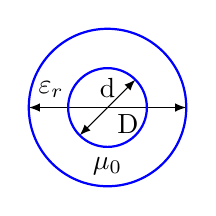
\begin{tikzpicture}
    \draw[latex-latex](-1,0)node[above right]{$\varepsilon_r$}--(1,0);
    \node[below right, yshift=1pt]{D};
    \draw[latex-latex, rotate=45](-0.5,0)--(.5,0);
    \node at (0,0)[above]{d};
    \draw[-, thick, blue](0,0) circle (1);
    \node at(0,-.75)[]{$\mu_0$};
    \draw[-, thick, blue](0,0) circle (0.5) ;
\end{tikzpicture}

\begin{align*}
    \Aboxed{Z_L &= \frac{Z_{F0}}{2\pi}\sqrt{\frac{\mu_r}{\varepsilon_r}}\ln\left( \frac{r_a}{r_i} \right)}  \overbrace{=}^{ \mu_r=1}\frac{60\Omega}{\sqrt{\varepsilon_r}}\cdot \ln{\frac{r_a}{r_i}}
\end{align*}

\subsubsection{Dämpfung}
Hin- und Rückleiter!\\
\underline{\textbf{Ohmsche Verluste}} $R\ll\omega L$
\[
    \alpha_L = \frac{\sqrt{\dfrac{f\cdot\mu}{\pi\cdot\kappa}}}{120\Omega}\cdot\frac{\sqrt{\varepsilon_r}}{D}\cdot\dfrac{1+\dfrac{D}{d}}{\ln \dfrac{D}{d}}
\]

Dämpfungsminimum für $ \frac{1+\tfrac{D}{d}}{\ln \tfrac{D}{d}} = 1 $\\ bei vorgegebenen Außendurchmesser: $ \frac{D}{d} =3,59 $\\

\underline{\textbf{Dielektrische Verluste}} $G\ll\omega C$,$\tan\delta= (^G/_{\omega C})$
\[
    \alpha_d = \frac{\sqrt{\varepsilon_r}\pi f}{c_0}\cdot\tan\delta \sim f
\]

\subsection{Mikrostreifenleiter}
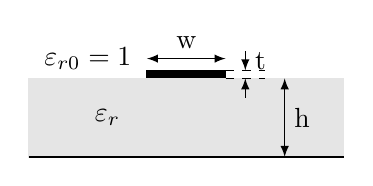
\begin{tikzpicture}
    %Leiterbahn
    \filldraw[black]    (1,1)   rectangle (2,1.1);
    %Dielektrika
    \filldraw[black!10] (-.5,0) rectangle (3.5,1);
    \draw[-,thick](-.5,0)--(3.5,0);
    %Bemassungen
    \draw[latex-latex](2.75,0)--(2.75,1) node[midway, right]{h};
    \draw[latex-latex](1,1.25)--(2,1.25) node[midway, above]{w};
    \draw[dashed](2,1)      --(2.5,1);
    \draw[dashed](2,1.1)    --(2.5,1.1);
    \draw[latex-](2.25,1)   --(2.25,.75);
    \draw[latex-](2.25,1.1) --(2.25,1.35) node[midway, right]{t};
    %Dielektrizitätskonstanten
    \node at (.5,.5)[]{$\varepsilon_r$};
    \node at (.25,1.25)[]{$\varepsilon_{r0}=1$};
\end{tikzpicture}

\subsubsection{Effektive Permittivitätszahl}
Unterschiedliche Phasengeschwindigkeit $\rightarrow$ Dispersion
\[
         \varepsilon_{r,\texttt{eff}}  = \frac{\varepsilon_r+1}{2}+\frac{\varepsilon_r-1}{2\sqrt{1+10\cdot\frac{\text{h}}{\text{w}}}} \\
\]

Je größer $\dfrac{\mathrm{w}}{\mathrm{h}}$ desto mehr nähert sich $\varepsilon_{r,\texttt{eff}}$ an $\varepsilon_r$ und 
\[
    \lambda = \frac{\lambda_0}{\sqrt{\varepsilon_{r,\texttt{eff}}\cdot\mu_{r,\texttt{eff}}}}
\]

\subsubsection[Schmale Streifen]{Schmale Streifen (ca 20-200$\Omega$)}
\[
    Z_L = \frac{60\Omega}{\sqrt{\varepsilon_{r,\texttt{eff}}}}\cdot\ln\left(\frac{8\mathrm{h}}{\mathrm{w}}+\frac{\mathrm{w}}{4\mathrm{h}}\right)
\]
\subsubsection[Breite Streifen]{Breite Streifen (ca 20-200$\Omega$)}
\[
    Z_L = \frac{120\pi\Omega}{\sqrt{\varepsilon_{r,\texttt{eff}}}}\cdot\frac{1}{\dfrac{\mathrm{w}}{\mathrm{h}}+2,42-0,44\cdot\dfrac{\mathrm{h}}{\mathrm{w}}+\left(1-\dfrac{\mathrm{h}}{\mathrm{w}}\right)^6}
\]

\subsection{Hohlleiter}
\[
    f_c = \frac{c_0}{2a}
\]

\subsection{VSWR (Voltage Standing Wave Ratio) und Return Loss}\label{sec:VSWR}

Überlagerung von einlaufender und reflektierender Welle. Wenn Transmission vorhanden $\rightarrow$ Teil der Welle wird an der Grenzfläche transmittiert. Abhängigkeit vom Reflexionsfaktor\\

\textbf{Reflexionsfaktor}\\
          \[ \underline{r}_2 = \underline{r}(z=0) = \frac{Z_2 - \underline{Z}_L}{Z_2 + \underline{Z}_L} \]
\underline{VSWR}
\begin{align*}
    s   & = \mathrm{VSWR} = \frac{1+|r|}{1-|r|}\geq 1 \\
    |r| & = \frac{s-1}{s+1}
\end{align*}
\underline{Return Loss}
\[
    \alpha_r = -20\log(r)dB
\]
\underline{Missmatch Loss}
\[
    \mathrm{ML} = -10\log(1-r^2)dB
\]
\subsection{Lichtwellenleiter oder Glasfaser}

\begin{description}
    \setlength\itemsep{1pt}
    \item APF := All Plastic Fiber
    \item POF := Polymerfaser
    \item LWL := Lichtwellenleiter
    \item $B\cdot l$ := Bandbreitenlängenprodukt
\end{description}

\begin{description}
    \item \underline{Dispersion:}

          {\small Die von der Frequenz des Lichts abhängende
              Ausbreitungsgeschwindigkeit des Lichts in Medien. Dies hat zur Folge,
              dass Licht an Übergangsflächen unterschiedlich stark gebrochen wird.
              Somit verflacht sich beispielsweise ein (Dirac-)Impuls zu einer Gauß'schen
              Glocke.
          }
    \item \underline{Stufenprofil:}

          {\small Multimode: leichtes Einkoppeln, geringes $B\cdot l$ wegen
              Modendispersion

              Single/Monomode: schwieriges Einkoppeln, großes $B\cdot l$, keine
              Modendispersion
          }
    \item \underline{Gradientenprofil:}

          {\small Multimode: Kompromiss beim Einkoppeln und Reichweite mit $B\cdot l$}
    \item \underline{Bandbreitenlängenprodukt:}

          {\small $B' =  B\cdot l[\frac{MHz}{km}]$ = konstant

              $B \sim \frac{1}{l}$ und $l\sim \frac{1}{B}$

              Bandbreite ist gegen Übertragungslänge austauschbar, solange
              Dämpfung keine Rolle spielt.
          }
\end{description}
\newpage
\subsection{Leitungsparameter}
\subsubsection{Streifenleitung / Parallele Platten}
Für Sinus-Anregung:
\begin{align*}
	I(l) & = \frac{U}{Z_L} = \underbrace{\frac{U_0}{Z_L}}_{I_0}\cdot e^{-j\beta l}\cdot e^{j\omega t}                     \\
	U(l) & = \int \vec{E} d\vec{s} \stackrel{b\gg d}{=} E\cdot d \rightarrow  &E = \frac{U_0}{d}\cdot e^{-j\beta l}\cdot\vec{e}_x \\
	I(l) & = \oint \vec{H} d\vec{s} =  H\cdot b \rightarrow &H = \frac{I_0}{b}\cdot e^{-j\beta l}\cdot\vec{e}_y                  % \\
	% \vec{E}(r, z) & = \frac{I}{2\pi r}\cdot Z_F\cdot e^{-j\beta z} \cdot\vec{e}_r                                                      \\
	%               & = \frac{\hat{U}}{r \cdot\ln{(^{2b}/_{2a})}}\cdot e^{-j\beta z}\cdot\vec{e}_r
\end{align*}
$ \mathbf{b} $: Platten\textbf{breite} \qquad $ \mathbf{d} $: Abstand zwischen den Platten\\

\begin{minipage}[t]{0.4\columnwidth}
\input{Figures/Leitungen_Parallele_Platten.tex}
\end{minipage}
\begin{minipage}[b][1cm]{0.6\columnwidth}
	\begin{flalign*}
		&R'=\frac{2}{\delta\kappa b}\left[ \frac{\Omega}{m} \right] & &L'=\frac{\mu d}{b} \left[\frac{H}{m}\right]&\\
		&G'=\frac{\kappa b}{d} \left[ \frac{S}{m} \right] &
		&C'=\frac{b\varepsilon}{d} \left[\frac{F}{m}\right]
	\end{flalign*}
\end{minipage}
%
%
%{\renewcommand*{\arraystretch}{0.2}
%	\begin{tabularx}{0.5\columnwidth}{X}
%		\hline
%		\[R'=\frac{2}{\delta\kappa b}\] \\
%		\hline
%		\[L'=\frac{\mu d}{b}\]         \\
%		\hline
%		\[G'=\frac{\kappa b}{d}\]      \\
%		\hline
%		\[C'=\frac{b\varepsilon}{d}\]  \\
%		\hline
%	\end{tabularx}
%}

\subsubsection{Doppelleitung}
$ \kappa $: Leitwert des Dielektrikums \qquad $ \kappa_L $ Leitwert des Leiters\\
$ \mathbf{r} $: Leiterradius \qquad $ \mathbf{d} $: Abstand zw. Leitermitten

\begin{minipage}[t]{0.4\columnwidth}
	\input{Figures/Leitungen_Doppelleitung.tex}
\end{minipage}
\begin{minipage}[b][4cm]{0.6\columnwidth}
	\begin{flalign*}
		&R'=\frac{1}{\pi a\delta\kappa_L} \left[ \frac{\Omega}{m} \right] &\\
		&L'= \frac{\mu}{\pi} \cosh^{-1}\frac{d}{2r} \left[\frac{H}{m}\right]&\\
		&G'= \frac{\pi\kappa}{\cosh^{-1}(^d/_{2r})} \left[ \frac{S}{m} \right] &\\
		&C'=\frac{\pi\varepsilon}{\cosh^{-1}(^d/_{2r})} \left[\frac{F}{m}\right]
	\end{flalign*}
\end{minipage}

%{\small\[
%	\text{cosh am TR: MENU $\rightarrow$ 1; OPTN $\rightarrow$ 1 $\rightarrow$ 5}\\
%	\]}
%\input{Figures/Leitungen_Doppelleitung.tex}
%{\renewcommand*{\arraystretch}{0.2}
%	\begin{tabularx}{0.5\columnwidth}{|X|}
%		\hline
%		\[R  = \frac{1}{\pi a\delta\kappa}\]              \\
%		\hline
%		\[L = \frac{\mu}{\pi} \cosh^{-1}\frac{d}{2a}\]      \\
%		\hline
%		\[G = \frac{\pi\kappa}{\cosh^{-1}(^d/_{2a})}\]      \\
%		\hline
%		\[C = \frac{\pi\varepsilon}{\cosh^{-1}(^d/_{2a})}\] \\
%		\hline
%\end{tabularx}}

\subsubsection{Koaxialleitung}
%{\small\[
%	a = \text{innen Radius} \qquad b = \text{außen Radius} \\
%	\]}
$ r_i $: Innenradius \quad $ r_a $: Außenradius
\begin{align*}
	\vec{H}(r, z)         & = \frac{\hat{I}}{2\pi r}\cdot e^{-j\beta z}\cdot\vec{e}_\varphi                   \\
	\vec{E}(r, z)         & = \frac{\hat{I}}{2\pi r}\cdot Z_{F0}\cdot e^{-j\beta z} \cdot\vec{e}_r
	& = \frac{\hat{U}}{r \cdot\ln{(^{r_a}/_{r_i})}}\cdot e^{-j\beta z}\cdot\vec{e}_r        \\
	S_{av} & = \frac{1}{2}\cdot\left( \frac{\hat{I}}{2\pi r}\right)^2\cdot Z_{F}
\end{align*}
\begin{minipage}[c][2cm]{0.4\columnwidth}
%	\input{Figures/Leitungen_Koaxialleitung.tex}
	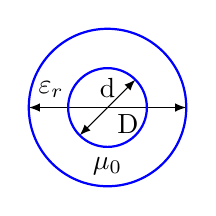
\begin{tikzpicture}
    \draw[latex-latex](-1,0)node[above right]{$\varepsilon_r$}--(1,0);
    \node[below right, yshift=1pt]{D};
    \draw[latex-latex, rotate=45](-0.5,0)--(.5,0);
    \node at (0,0)[above]{d};
    \draw[-, thick, blue](0,0) circle (1);
    \node at(0,-.75)[]{$\mu_0$};
    \draw[-, thick, blue](0,0) circle (0.5) ;
\end{tikzpicture}

\end{minipage}
\begin{minipage}[c][4cm]{0.6\columnwidth}
	\begin{flalign*}
		&R'=\frac{1}{2\pi\delta\kappa_L}\left(\frac{1}{r_a}+\frac{1}{r_i}\right) \left[ \frac{\Omega}{m} \right] &\\
		&L'=\frac{\mu_0\mu_r}{2\pi}\ln\frac{r_a}{r_i} \left[\frac{H}{m}\right]&\\
		&G'=\frac{2\pi\kappa}{\ln(r_a/r_i)} \left[ \frac{S}{m} \right] &\\
		&C'=\frac{2\pi\varepsilon_0 \varepsilon_r}{\ln(r_a/r_i)} \left[\frac{F}{m}\right]
	\end{flalign*}
\end{minipage}
%
%
%{\renewcommand*{\arraystretch}{0.2}
%	\begin{tabularx}{0.5\columnwidth}{|X|}
%		\hline
%		\[R=\frac{1}{2\pi\delta\kappa_c}\left[\frac{1}{a}+\frac{1}{b}\right]\] \\
%		\hline
%		\[L=\frac{\mu}{2\pi}\ln\frac{b}{a}\]                                   \\
%		\hline
%		\[G=\frac{2\pi\kappa}{\ln(^b/_a)}\]                                    \\
%		\hline
%		\[C=\frac{2\pi\varepsilon}{\ln(^b/_a)}\]                               \\
%		\hline
%\end{tabularx}}
\vspace{1ex}
\subsubsection{Allgemein}
Für beliebige Leitergeometrie gelten folgende Zusammenhänge:
\[
LC = \mu\varepsilon \quad \text{und} \quad \frac{G}{C} = \frac{\kappa}{\varepsilon}
\]
Innere Induktivität:
\[
L_i = \frac{R}{w}
\]
\textbf{\color{red}{Leitungen gehen HIN und ZURÜCK!!!}\\
	\color{red}{Länge verdoppeln!!!}
}
	\section{Smith-Diagramm}

\subsection{Allgemein} \label{sec:Smith_All}


%$m$             : Anpassungsfaktor
%
%$s$             : inverser Anpassungsfaktor
%
%$\underline{r}$ : Reflexionsfaktor
%
%$1$             : Anpassungspunkt

\subsubsection{Normierte Impedanz}
\begin{align*}
	\underline{z}_n= \frac{Z(l)}{Z_L} = \frac{Z_2+jZ_L\cdot\tan(\beta l)}{Z_L+jZ_2\cdot\tan(\beta l)}
\end{align*}


\subsubsection{Reflexionsfaktor}
%$ \underline{U}_r(l) = \underline{U}_r(l=0) \cdot e^{-j\beta l} \qquad \underline{U}_h(l) = \underline{U}_h(l=0) \cdot e^{j\beta l} $
$ \underline{r}(l) = \underline{r} \qquad \underline{r}_{(l=0)} = \underline{r}_2 \qquad 0<r<1 \qquad 0<\Psi<2\pi $
Immer gültig, auch ohne Quelle!
\begin{flalign*}
	\underline{r} &= \underline{r}_2 \cdot e^{-j2\beta l} = r \cdot e^{-j(\Psi_0+2\beta l)} =r\cdot e^{j\Psi} \\ &=\frac{\underline{z}_n-1}{\underline{z}_n+1}\\
	\underline{r}_2 & = \frac{\underline{Z}_2-Z_L}{\underline{Z}_2+Z_L} = \frac{\underline{U}_2-\underline{I}_2Z_L}{\underline{U}_2 +\underline{I}_2 Z_L}\\
	 \underline{z}_n & = \frac{1+\underline{r}}{1-\underline{r}}
\end{flalign*}
%    \begin{align*}
%        \Aboxed{ \underline{z}'(l) = \frac{Z(l)}{Z_L} = \frac{Z_2+jZ_L\cdot\tan(\beta l)}{Z_L+jZ_2\cdot\tan(\beta l)}} \\
%        \text{mit} \beta = \frac{2\pi}{\lambda}                                                \\
%        \text{auch ohne Quelle gültig!}
%    \end{align*}

\subsubsection{Anpassungsfaktor}
Werte von $ m \rightarrow$ Werte von $ \Re{\underline{z}_n}: 0 \leq m \leq1 $
\begin{align*}
	m = \frac{U_{min}}{U_{max}} = \frac{I_{min}}{I_{max}}=\frac{1-|\underline{r}|}{1+|\underline{r}} \qquad  |\underline{r}| = \frac{1-m}{1+m} \qquad s=\frac{1}{m}
\end{align*}
\begin{center}
    \input{Figures/Smithdiagramm_Smithchart.tex}
\end{center}
\begin{align*}
    \underline{z}_n & = \frac{\underline{Z}_n}{Z_L}                                                                                                                   \\
    \underline{r}_n & = \frac{\underline{Z}_n-Z_L}{\underline{Z}_n+Z_L}= \frac{\underline{z}_n-1}{\underline{z}_n+1}    = \frac{1-\underline{y}_n}{1+\underline{y}_n} \\
    m               & = \frac{1-|\underline{r}|}{1+|\underline{r}|}                                                                                                   \\
    s               & = \frac{1}{m} = \mathrm{SWR}       = \frac{U_\text{max}}{U_\text{min}} = \frac{I_\text{max}}{I_\text{min}} = \frac{1+|r(l)|}{1-|r(l)|} = \frac{|U_h|+|U_r|}{|U_h|-|U_r|}= \dfrac{R_{\text{max}}}{Z_L}
\end{align*}

\subsection{Impedanz/Admetanz umrechnen}
Spiegelung von $ \underline{z}_n $ um Mittelpunkt ergibt $ \underline{y}_n $.  (Phase $\pm 180^{\circ}$/$\pm \pi$)

%\subsection{Zusammenschaltungen}
% \begin{center}
%     \includegraphics[width=.45\columnwidth]{Figures/Smithdiagramm_Zusammenschaltungen.png}
% \end{center}

%\columnbreak

\subsection{Maxima und Minima bei stehender Welle}
Bei \textbf{verlustloser} Leitung:
\begin{align*}
	&U_{\texttt{max}} = |U_h| \cdot (1+|r(l)|) & U_{\texttt{min}} = |U_h| \cdot (1-|r(l)|) &\\
	&I_{\texttt{max}} = \left | \frac{U_h}{Z_L} \right | \cdot (1+|r(l)|) & I_{\texttt{min}} = \left| \frac{U_h}{Z_L} \right | \cdot (1-|r(l)|) &
\end{align*}
Für Spannungen: Abstand von der Last $ z $ 
\begin{align*}
	 &z_{\texttt{min}} = \frac{\lambda}{4\pi}(\theta_{rad}+(2n+1)\pi)&
	 z_{\texttt{max}} = \frac{\lambda}{4\pi} \cdot (\theta_{rad}+2n\pi)&\\
	 &\text{\textbf{Minima} alle}\: \frac{\lambda}{2} &
	 \text{\textbf{Maxima} alle}\: \frac{\lambda}{4} &
\end{align*}

\subsection[Von Last zu Quelle]{Lastseite $\rightarrow$ Quelle}
\begin{enumerate}
    \item $Z_L = Z_B$ ins Diagramm einzeichnen
    \item Lastimpedanz bestimmen,
          wenn z.B. Parallelschaltung etc.
    \item Normieren
          \[\underline{z}_n = \frac{\underline{Z}(l)}{Z_L} \]
    \item Im Chart eintragen
    \item Linie vom Mittelpunkt durch $\underline{z}_ns$ nach außen

          Ablesen und Notieren:

          $\rightarrow$ Relative Länge $\left[\frac{l}{\lambda}\right]$

          $\rightarrow$ Relativer Winkel in \textbf{Degree}
    \item Kreis einzeichen

          Ablesen und Notieren:

          $\rightarrow$ \textbf{Maxima}: rechter Schnittpunkt mit Re-Achse

          $\rightarrow$ \textbf{Minima}: linker Schnittpunkt mit Re-Achse

          $\rightarrow$ $ \underline{r} $ abmessen und aus oberer Skala auslesen
    \item Um Leitungslänge im UZS laufen
          $\rightarrow$ Linie vom Mittelpunkt durch neuen Punkt nach außen

          Ablesen und Notieren:

          $\rightarrow$Relativer Winkel
    \item Wenn $\alpha\neq 0$

          $\rightarrow$ Dämpung ausrechen
          $\rightarrow$ Um Faktor nach innen Spiralieren

    \item Dieser Punkt ist $\underline{z}_e$
    \item Eingangsimpedanz ablesen
          \[\underline{Z}_E = \underline{z}_e \cdot Z_L\]
\end{enumerate}


\usetikzlibrary{decorations.pathmorphing}
\usetikzlibrary{decorations.text}
\tikzset{
cross/.style={cross out, draw=black, minimum size=2*(#1-\pgflinewidth), inner sep=0pt, outer sep=0pt},
%     %default radius will be 1pt. 
cross/.default={3.5pt}
dot/.style={circle, fill=#1, inner sep=0, minimum size=4pt},
mini dot/.style={circle, inner sep=0pt, minimum size=2pt, pos=1, fill, node contents={}},
}
\begin{center}
 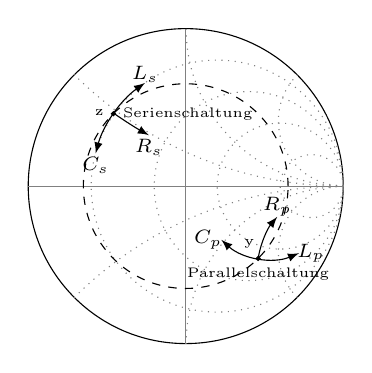
\begin{tikzpicture}    
    
    %Außenkreis
    \draw[-](0,0) circle (2);

    %Realteil Linien
    \draw[-, black!50](-2,0)--(2,0);

    \draw[dotted, black!50](0.4,0) circle (1.6);
    \draw[dotted, black!50](0.8,0) circle (1.2);
    \draw[dotted, black!50](1.2,0) circle (0.8);
    \draw[dotted, black!50](1.6,0) circle (0.4); 

    
    %Imaginärteil Linien
    \draw[-, black!50](0,-2)--(0,2);

    \draw[dotted, black!50, xshift = 13.25ex, yshift = -31.98ex](135:4.84)arc(135:90:4.84);
    \draw[dotted, black!50, xshift = 13.25ex, yshift = -13.25ex](180:2)   arc(180:90:2);
    \draw[dotted, black!50, xshift = 13.25ex, yshift = -5.485ex](225:.828)arc(225:90:.828);

    \draw[dotted, black!50, xshift = 13.25ex, yshift = 31.98ex](270:4.84)arc(270:225:4.84);
    \draw[dotted, black!50, xshift = 13.25ex, yshift = 13.25ex](270:2)   arc(270:180:2);
    \draw[dotted, black!50, xshift = 13.25ex, yshift = 5.485ex](270:.828)arc(270:135:.828);

    %Reflexionsfaktorkreis
    \draw[dashed](0,0) circle (1.3);

    %Serienschaltung
    \draw[-,fill=black!100] (-.919,.919) circle (0.025)node[left, yshift =.5] {\tiny z}node[right]{\tiny Serienschaltung};
    \draw[latex-latex, xshift = 2.65ex](125:1.6)node[above, yshift=-.75ex]{\scriptsize${L_s}$} arc (125:165:1.6)node[below, yshift=.5ex]{\scriptsize$C_s$};
    \draw[latex-, xshift = 13.25ex, yshift = 33.75ex](241:5.1)node[below, yshift=.5ex]{\scriptsize$R_s$}arc(241:235:5.1);

    %Parallelschaltung
    \draw[-,fill=black!100] (.919,-.919) circle (0.025)node[above left, xshift = .5ex]{\tiny y} node[below]{\tiny Parallelschaltung};
    \draw[-latex, xshift = 13.25ex, yshift = -7.25ex](170:1.1)arc(170:140:1.1)node[above, yshift=-.75ex]{\scriptsize$R_p$};

    \draw[latex-latex, xshift = 7.12ex](293:.925)node[right, xshift = -.95ex]{\scriptsize$L_p$}arc(293:227.5:.925)node[left, xshift = .85ex]{\scriptsize$C_p$};

\end{tikzpicture}
\end{center}  
	\section{Antennen}
\subsection{Herz'scher Dipol}
\subsubsection{Nahfeld: $r \ll \lambda$}

Überwiegend \textbf{Blindleistungsfeld}, da $E$ zu $H$ $90^\circ$
phasenverschoben
\begin{align*}
    H & = \vec{\Phi}\cdot\frac{I_0 \Delta l}{4\pi R^2}\cdot \sin\Theta                                                \\
    E & = \frac{I_0 \Delta l}{4\pi j \omega\varepsilon R^3}(2\vec{R} \cdot \cos\Theta + \vec{\Theta}\cdot \sin\Theta)
\end{align*}

\begin{align*}
    E_r       & = \frac{I l \lambda}{4\pi^2\varepsilon_0  c_0}\cdot \frac{1}{r^3} \cdot\cos\upsilon \cdot \sin(\omega t - \beta r) \\
    E_v       & = \frac{I l \lambda}{4\pi^2\varepsilon_0  c_0}\cdot \frac{1}{r^3} \cdot\sin\upsilon \cdot \sin(\omega t - \beta r) \\
    H_\varphi & = \frac{I l}{4\pi}\cdot \frac{1}{r^2}\cdot\sin\varphi\cdot\cos(\omega t -\beta r)
\end{align*}

\subsubsection{Fernfeld: $r \gg \lambda$}

Überwiegend \textbf{Wirkleistungsfeld}, $\vec{S}$ nach außen somit Kugelwelle

\vspace{1ex}
mit $\eta = Z_{F0}$

\begin{empheq}[box=\fbox] {align*}
    H & = \vec{\Phi}\cdot j\frac{\beta I_0 \Delta l}{4\pi R}\cdot \sin\Theta                             \\
    E & = \vec{\Theta}\cdot j\frac{\beta I_0 \Delta l }{4\pi R} \cdot \sin\Theta \cdot\eta e^{-j\beta R}
\end{empheq}

\begin{align*}
    E_r       & = 0                                                                                                           \\
    E_v       & = -\frac{I l }{2\varepsilon_0  c_0 \lambda}\cdot \frac{1}{r} \cdot\sin\upsilon \cdot \sin(\omega t - \beta r) \\
    H_\varphi & = -\frac{I l}{2\lambda}\cdot \frac{1}{r}\cdot\sin\upsilon\cdot\sin(\omega t -\beta r)
\end{align*}

\subsubsection{Abgestrahlte Leistung im Fernfeld}
\begin{align*}
    P_{rad} = \frac{\eta {I_0}^2 \beta^2 (\Delta l')^2}{12\pi} = \frac{I_0^2\eta\pi}{3}\cdot \dfrac{\Delta l'^2}{\lambda^2}
\end{align*}

\subsection{Bezugsantennen}
\[
    \boxed{g = 10 \cdot log(G)dB}
\]

mit $P_0$ : Eingangsleistung der Antenne

\begin{description}
    \item \textbf{\underline{G$\rightarrow$Bezugsantenne:}}

          Elementardipol  zu Kugelstrahler \[D = 1,50 \rightarrow g = 1,76\si{dBi}\]
          Halbwellendipol zu Kugelstrahler \[D = 1,64 \rightarrow g = 2,15\si{dBi}\]

    \item \textbf{\underline{EIRP}: Eqivalent \underline{Isoropic} Radiated Power}
          \[
              \text{EIRP} = P_0 \cdot G_i [dBi]
          \]

    \item \textbf{\underline{ERP}: Eqivalent Radiated Power (verlustloser Halbwellendipol)}
          \[
              \text{ERP} = P_0 \cdot G_d [dBd]
          \]
\end{description}

\end{multicols*}
\section{Antennen}
\begin{minipage}{1.7\columnwidth}
    \includegraphics[width=.55\columnwidth]{Figures/Antennentabelle_1.png}\\
    \includegraphics[width=.55\columnwidth]{Figures/Antennentabelle_2.png}
\end{minipage}
\section{Einheiten}
% \begin{table}
\begin{NiceTabular}{c|l|l}[cell-space-limits=3pt]
    \hline
    Symbol & Größe & Einheit\\
    \hline 
    A, W & Arbeit, Energie & J = VAs = Ws\\
    $\vec{A}$ & mag. Vektorpotenzial & $\dfrac{Vs}{m} = \dfrac{Wb}{m}$ ($\vec{B}$ = $\nabla \times \vec{A}$)\\
    $\vec{B}$ & mag. Flussdichte & $T = \dfrac{Vs}{m^2}$\\
    C & Kapazität & $F = \dfrac{As}{V}$\\
    $\vec{D}$ & dielek. Verschiebung/Erregung & $\dfrac{As}{m^2}$\\
    e, q, Q & (Elementar-)ladung & C = As\\
    $\vec{E}$ & elek. Feldstärke & $\dfrac{V}{m}$ \\
    $\vec{H}$ & mag. Feldstärke/Erregung & $\dfrac{A}{m}$\\
    $\vec{J}$ & Stromdichte & $\dfrac{A}{m^2}$\\
    $\vec{J}_F$ & Flächenstromdichte & $\dfrac{A}{m}$\\
    $\vec{M}$ & Drehmoment & J = Nm = VAs\\
    F & Kraft & $\dfrac{kgm}{s} = N$\\
    $R_{mag}$ & mag. Widerstand & $\dfrac{S}{s} = \dfrac{A}{Vs}$\\
    $\vec{S}$ & Poynting-Vektor & $\dfrac{W}{m^2}$\\
    Z & Wellenwiderstand & $\Omega$\\
    $\delta_s$ & Eindringtiefe & m \\
    $\varepsilon$ & Dielektrizitätskonstante & $\dfrac{As}{Vm}$\\
    $\varphi$ & elek. Skalarpotenzial & V \\
    $\varphi_m$ & mag. Skalarpotenzial & A \\
    $\rho$ & Raumladungsdichte & $\dfrac{As}{m^3}$\\
    $\rho$ & spez. Widerstand & $\dfrac{\Omega}{m} = \dfrac{VA}{m}$\\
    $\kappa, \sigma$ & elek. Leitfähigkeit & $\dfrac{S}{m} = \dfrac{A}{Vm}$\\
    $\lambda$ & Wellenlänge & m\\
    $\mu$ & Permiabilitätskonstante & $\dfrac{Vs}{Am}$\\
    $\Phi_e$ & elek. Fluss & C = As\\
    $\Phi_m$ & mag. Fluss & $Wb = \dfrac{T}{m^2}$\\

    \hline
\end{NiceTabular}
% \end{table}
    


\end{document}
